
\appendix

\chapter{Appendix Title}
\label{sec:appendix1}

Experiment for comparing time complexity that performed on large models:
\begin{figure}[H]
        \centering

        \begin{subfigure}[b]{0.5\textwidth}
                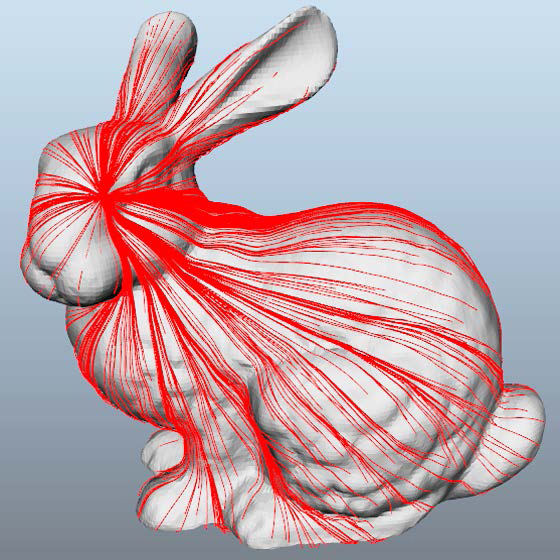
\includegraphics[width=\textwidth]{../images/geodesic_image/bunny}
                \caption{geodesics on bunny}
                \label{fig:bunny}
        \end{subfigure}%
        ~ %add desired spacing between images, e. g. ~, \quad, \qquad etc.
          %(or a blank line to force the subfigure onto a new line)
        \begin{subfigure}[b]{0.5\textwidth}
                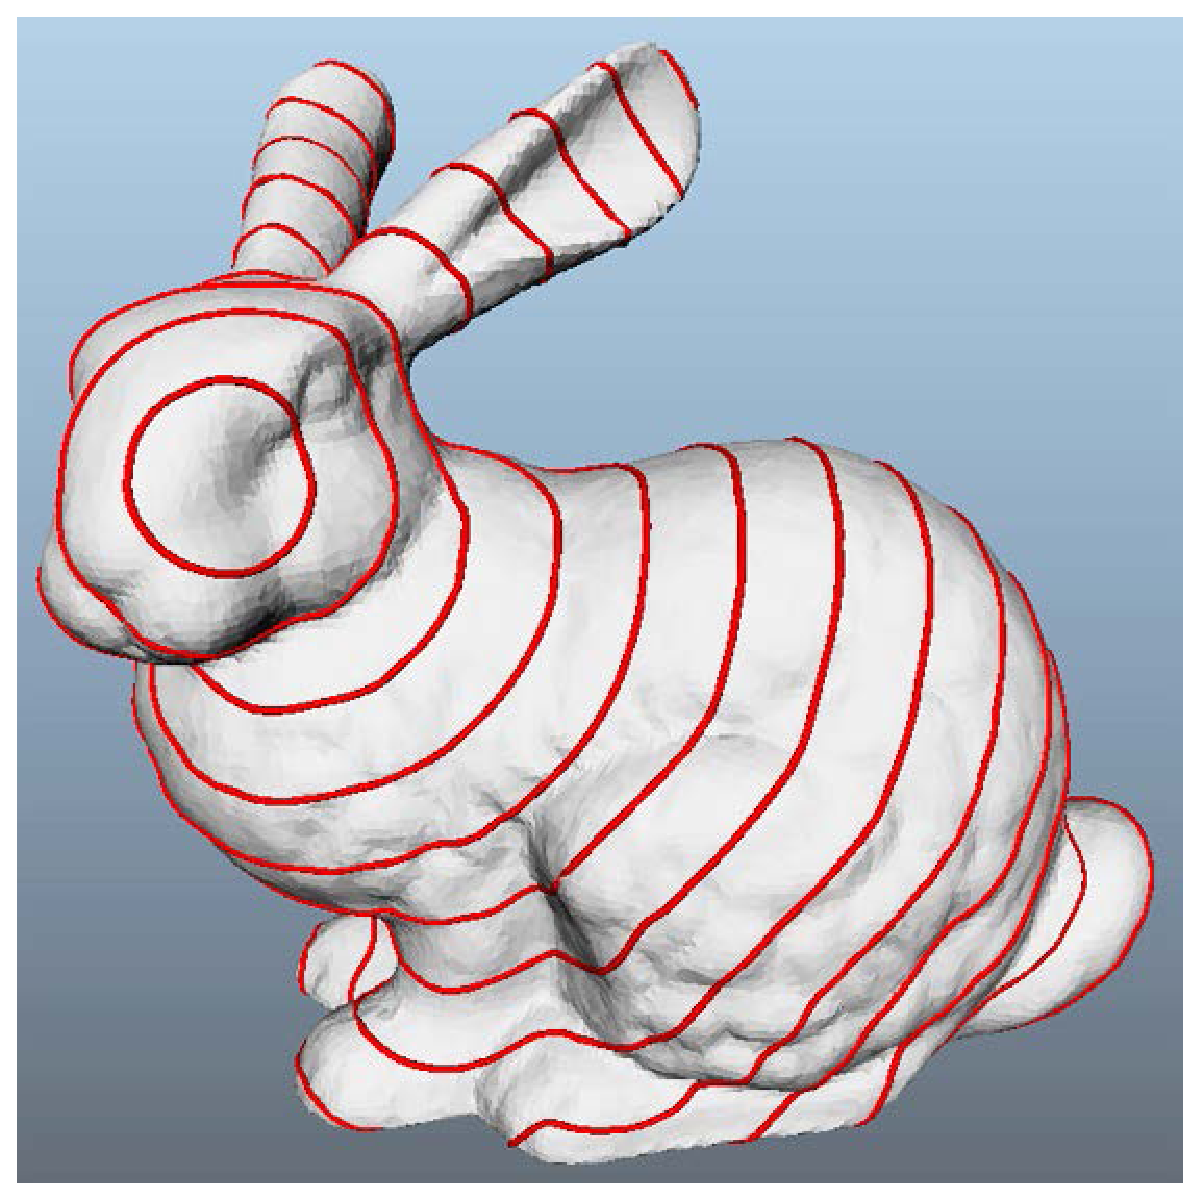
\includegraphics[width=\textwidth]{../images/geodesic_image/bunny_isoline}
                \caption{isoline on bunny}
                \label{fig:bunny_iso}
        \end{subfigure}
        
        \begin{subfigure}[b]{0.5\textwidth}
                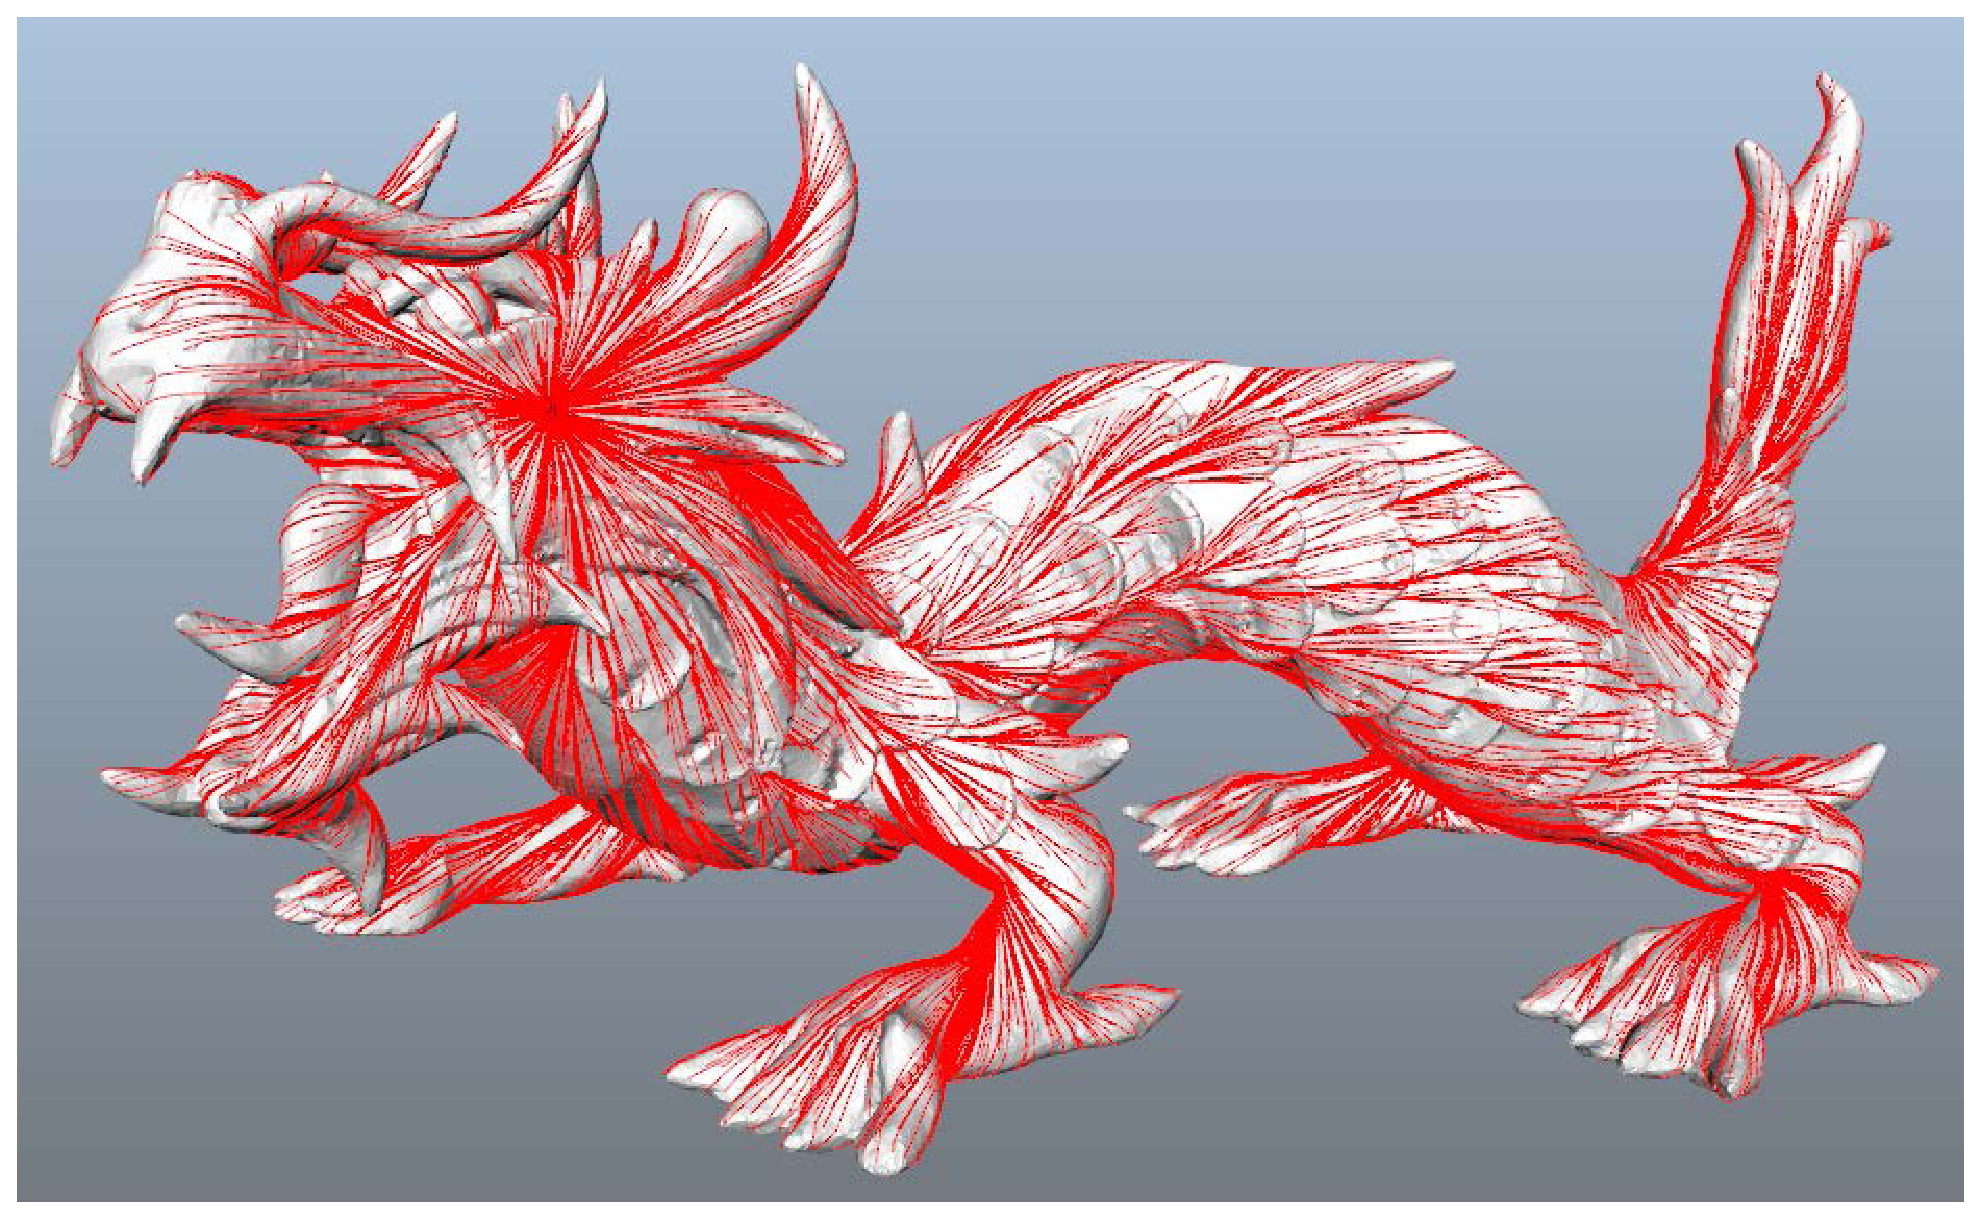
\includegraphics[width=\textwidth]{../images/geodesic_image/asian_dragon}
                \caption{geodesics on asian dragon}
                \label{fig:asian_dragon}
        \end{subfigure}%
        ~ %add desired spacing between images, e. g. ~, \quad, \qquad etc.
          %(or a blank line to force the subfigure onto a new line)
        \begin{subfigure}[b]{0.5\textwidth}
                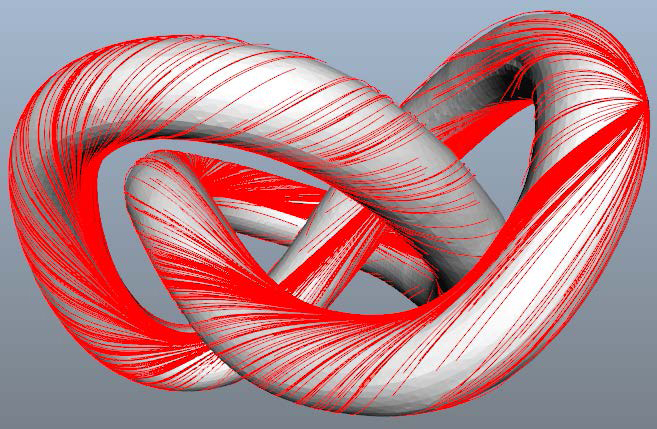
\includegraphics[width=\textwidth]{../images/geodesic_image/knot-1}
                \caption{geodesics on knot}
                \label{fig:knot}
        \end{subfigure}	             
\end{figure}


\begin{figure}
		\ContinuedFloat
        \centering

        \begin{subfigure}[b]{0.5\textwidth}
                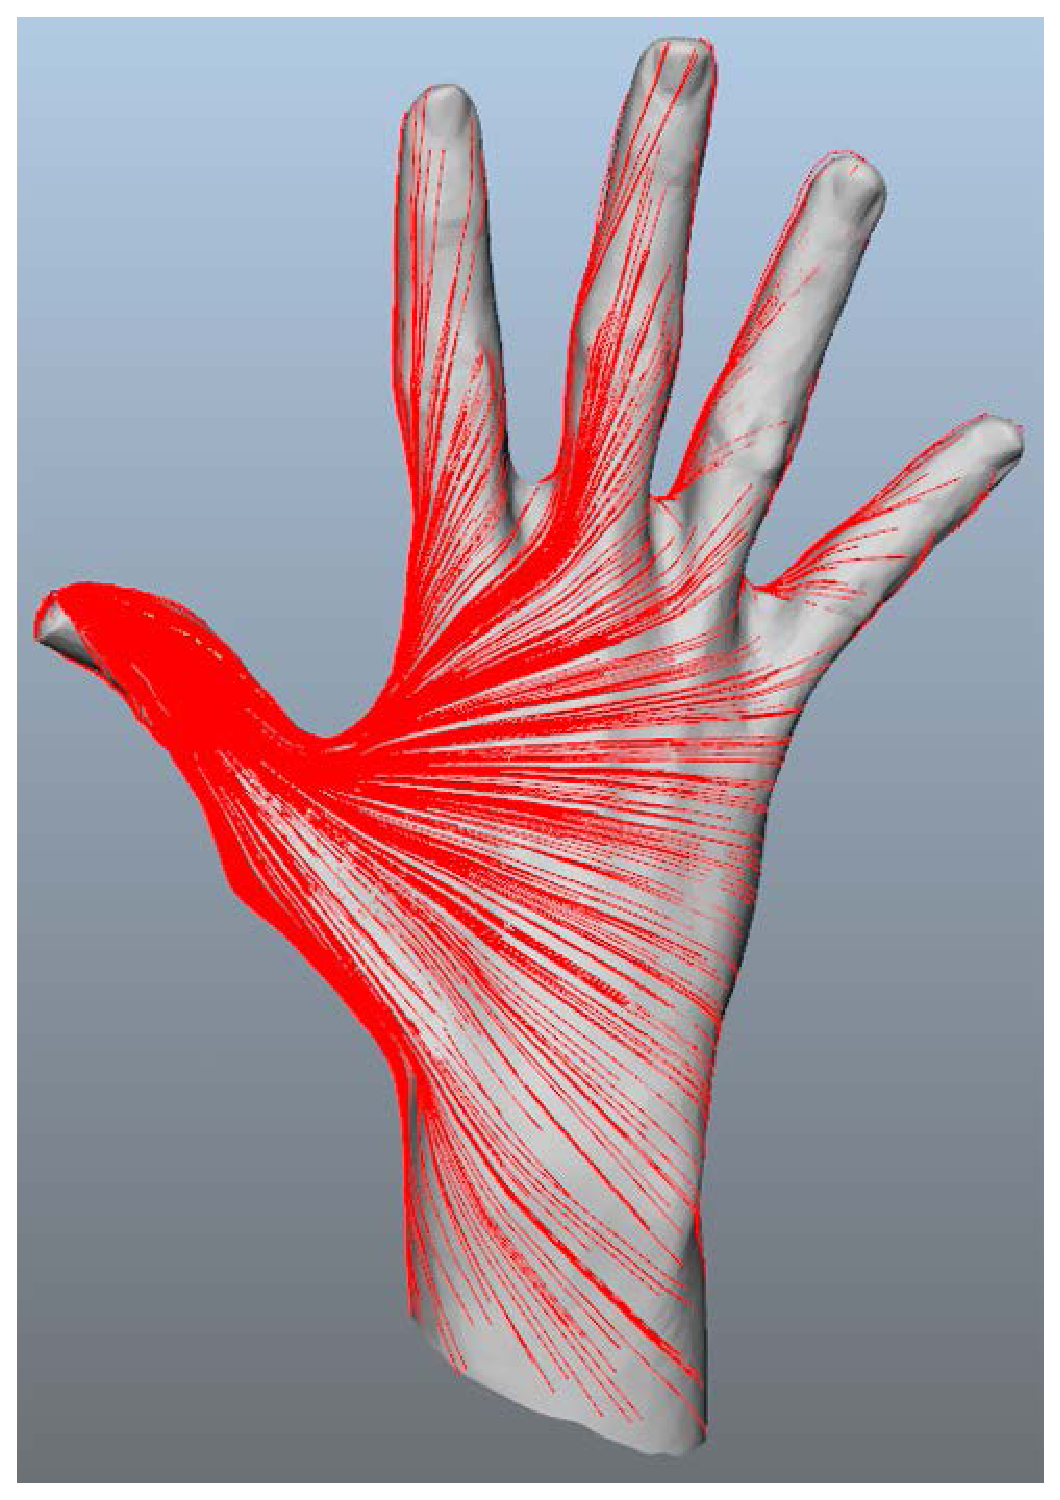
\includegraphics[width=\textwidth]{../images/geodesic_image/hand2-1}
                \caption{geodesics on hand}
                \label{fig:hand}
        \end{subfigure}%
        ~ %add desired spacing between images, e. g. ~, \quad, \qquad etc.
          %(or a blank line to force the subfigure onto a new line)
        \begin{subfigure}[b]{0.5\textwidth}
                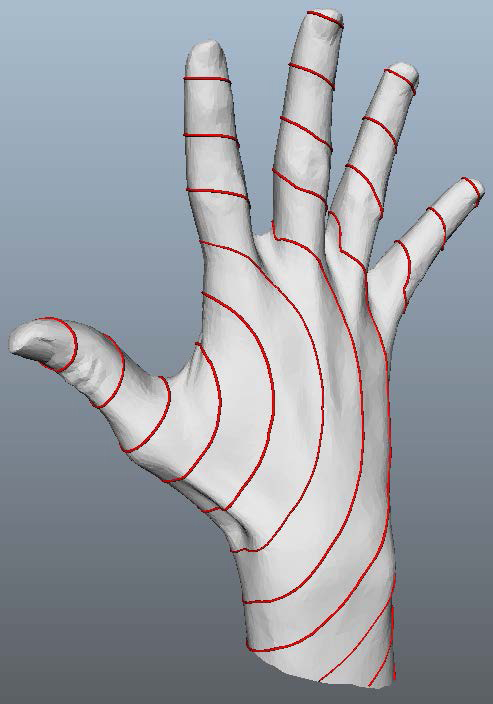
\includegraphics[width=\textwidth]{../images/geodesic_image/hand_isoline-1}
                \caption{isoline on hand}
                \label{fig:hand_iso}
        \end{subfigure}
        
         \begin{subfigure}[b]{0.5\textwidth}
                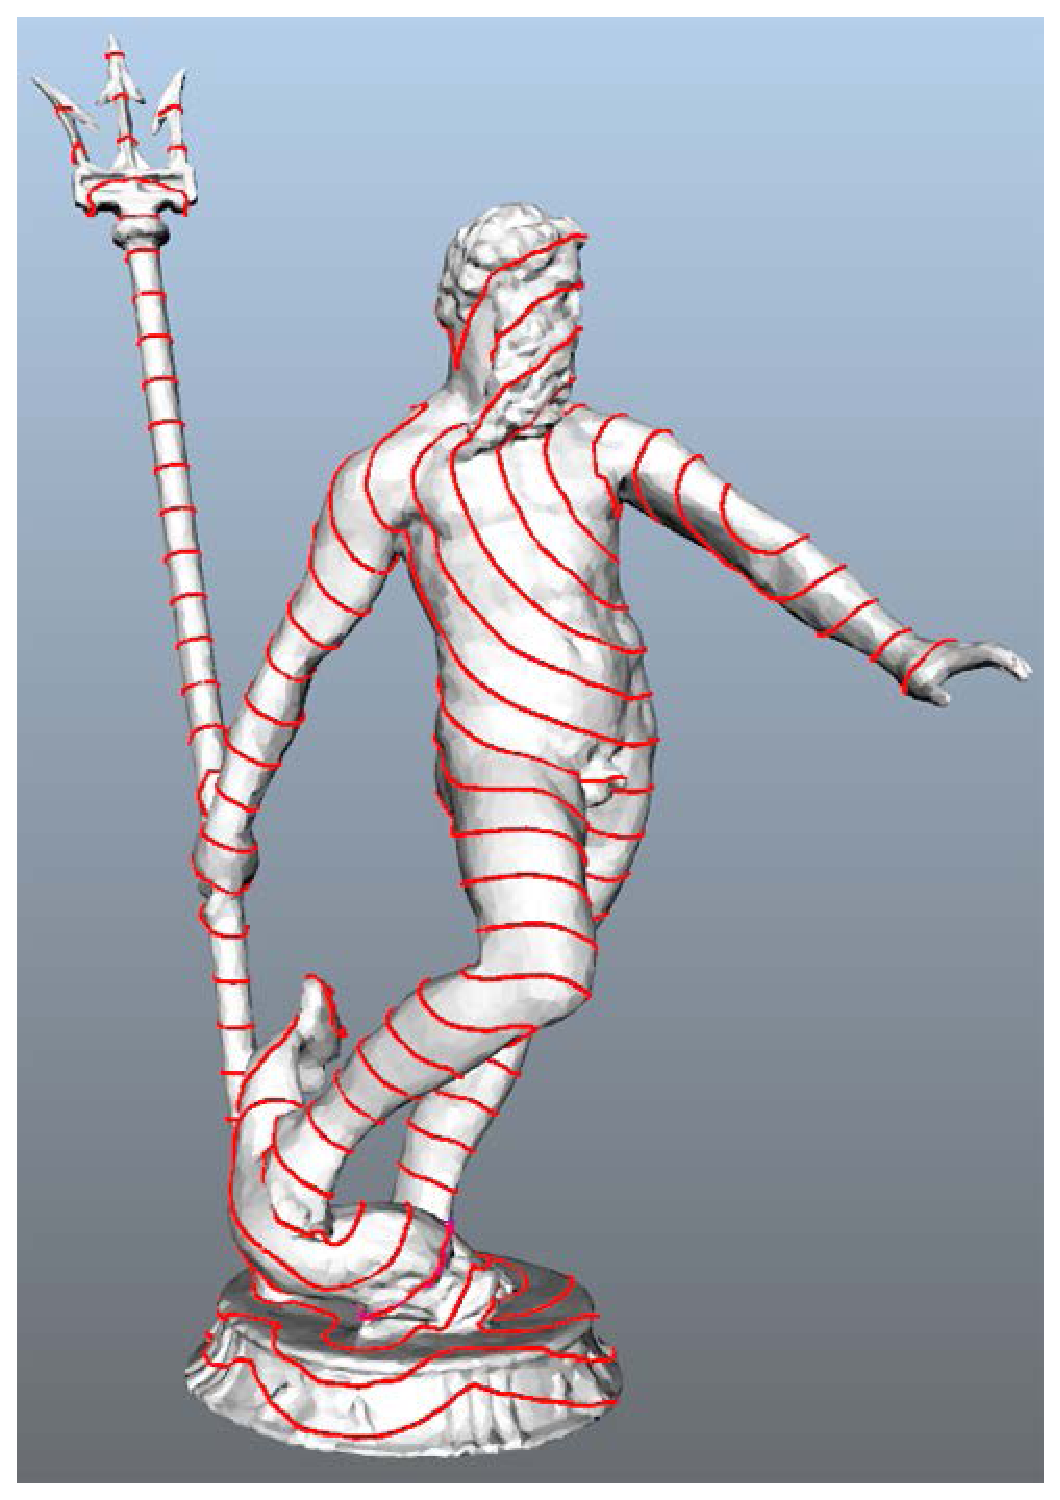
\includegraphics[width=\textwidth]{../images/geodesic_image/neptune1-1}
                \caption{geodesics on Neptune}
                \label{fig:neptune}
        \end{subfigure}%
        ~
        \begin{subfigure}[b]{0.5\textwidth}
                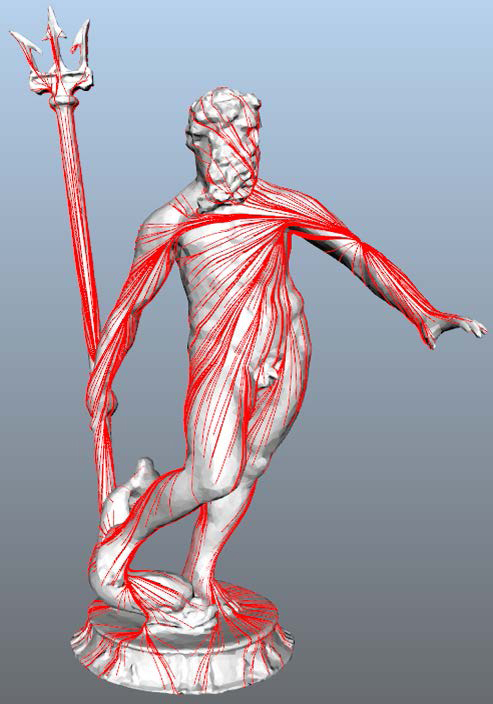
\includegraphics[width=\textwidth]{../images/geodesic_image/neptune_path-1}
                \caption{isoline on Neptune}
                \label{fig:neptune_iso}
        \end{subfigure}%        
\end{figure}


\begin{figure}
		\ContinuedFloat
        \centering

        \begin{subfigure}[b]{0.5\textwidth}
                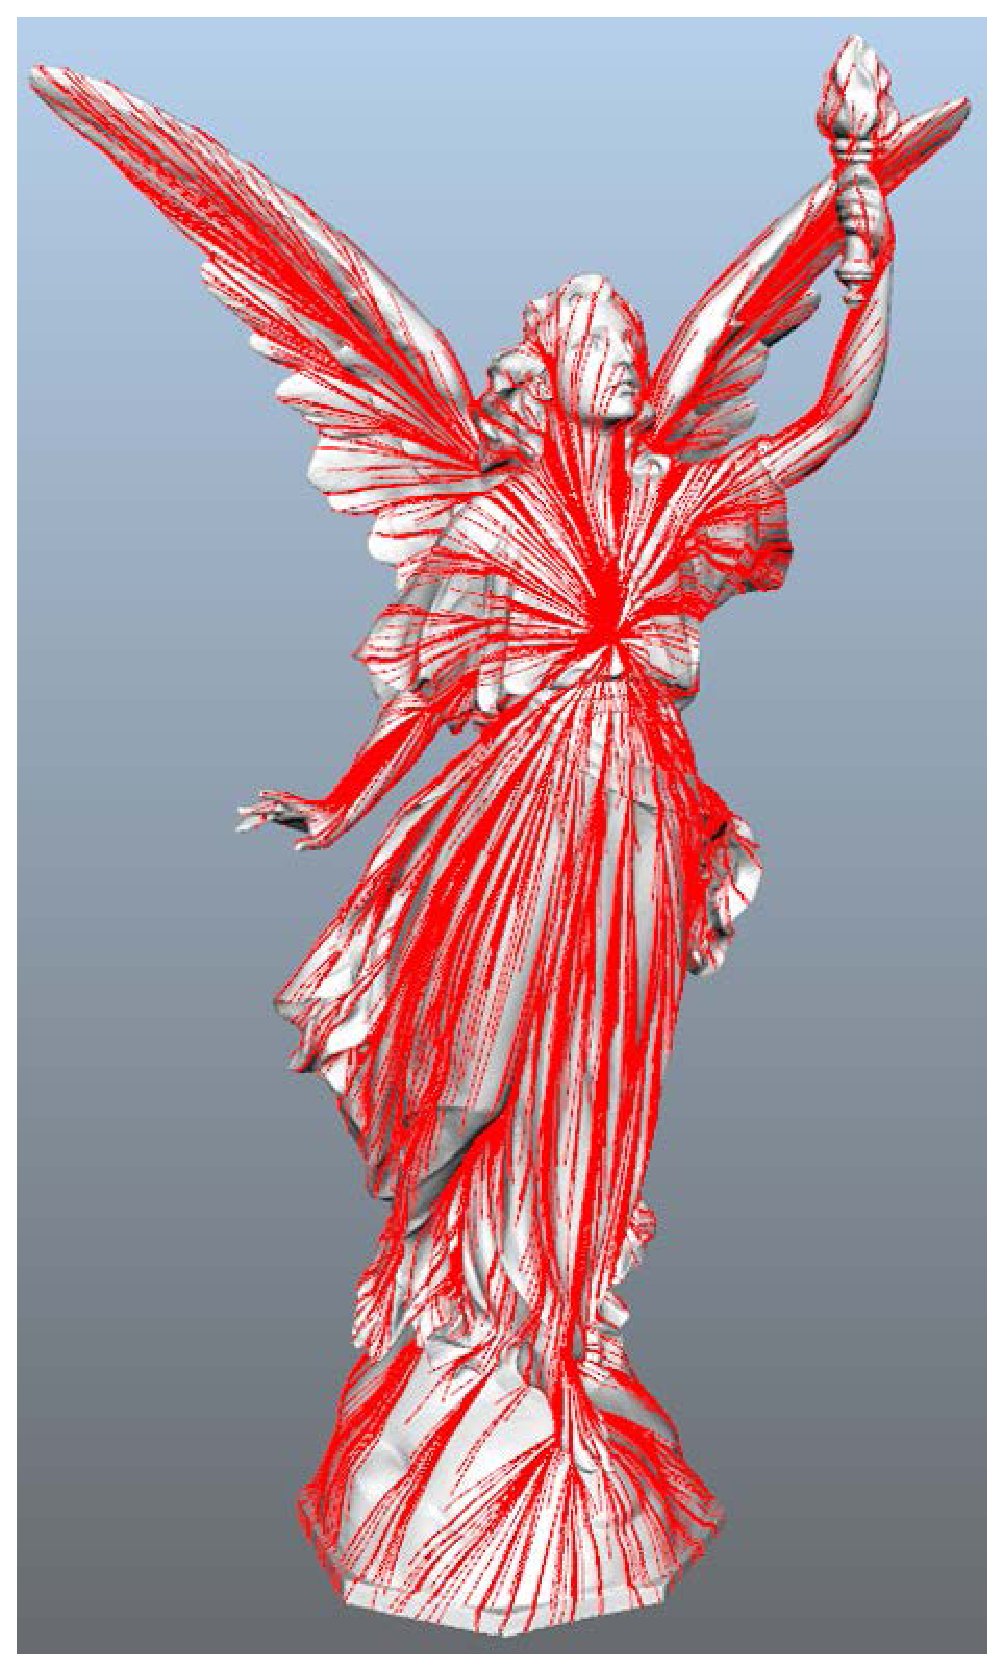
\includegraphics[width=\textwidth]{../images/geodesic_image/lucy_allpath-1}
                \caption{geodesics on Lucy}
                \label{fig:lucy}
        \end{subfigure}%
        ~
        \begin{subfigure}[b]{0.5\textwidth}
                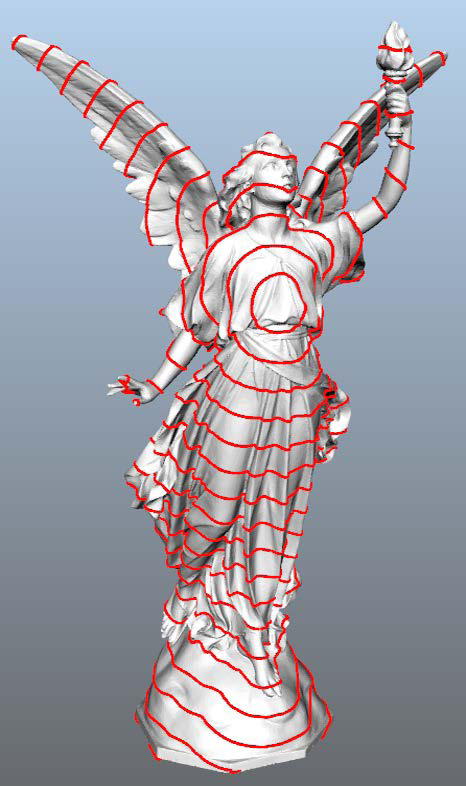
\includegraphics[width=\textwidth]{../images/geodesic_image/lucy_iso-1}
                \caption{isoline on Lucy}
                \label{fig:lucy_iso}
        \end{subfigure}%     


        \begin{subfigure}[b]{0.5\textwidth}
                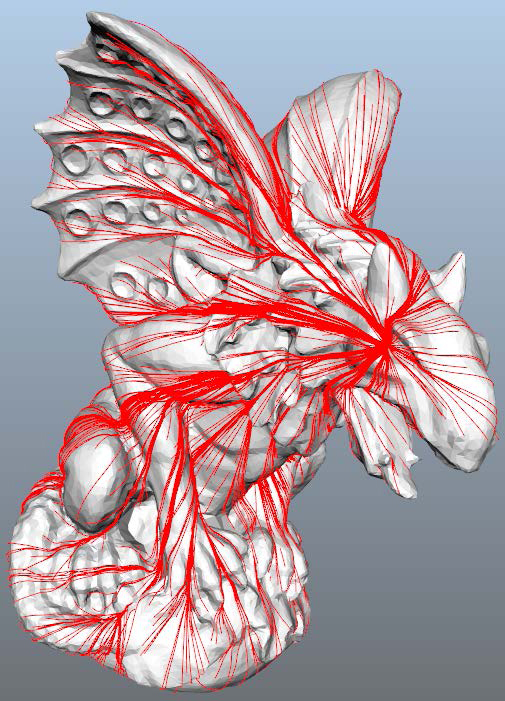
\includegraphics[width=\textwidth]{../images/geodesic_image/gargo2-1}
                \caption{geodesics on Gargoyle}
                \label{fig:gargo}
        \end{subfigure}%
        ~ %add desired spacing between images, e. g. ~, \quad, \qquad etc.
          %(or a blank line to force the subfigure onto a new line)
        \begin{subfigure}[b]{0.5\textwidth}
                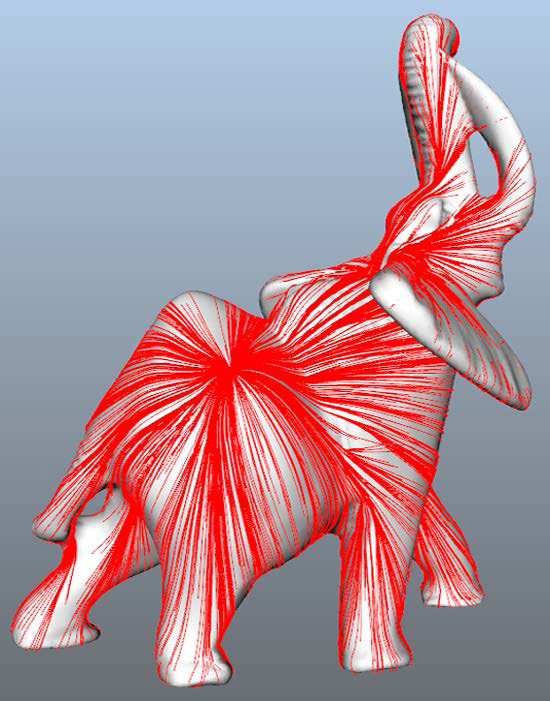
\includegraphics[width=\textwidth]{../images/geodesic_image/elephant-1}
                \caption{isoline on elephant}
                \label{fig:elephant}
        \end{subfigure}        
\end{figure}


 \begin{figure}
 		\ContinuedFloat
        \centering       
        
         \begin{subfigure}[b]{0.5\textwidth}
                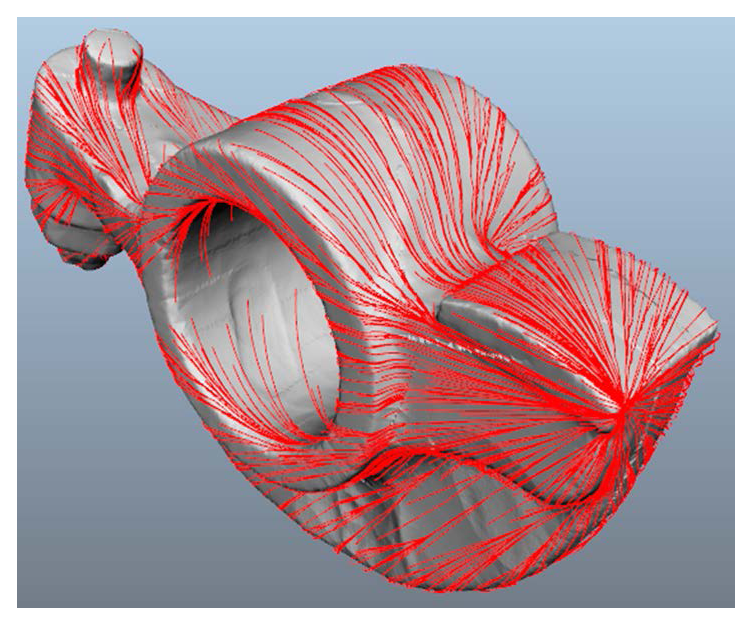
\includegraphics[width=\textwidth]{../images/geodesic_image/rock_arm}
                \caption{geodesics rockarm}
                \label{fig:rockarm}
        \end{subfigure}%
        ~
        \begin{subfigure}[b]{0.5\textwidth}
                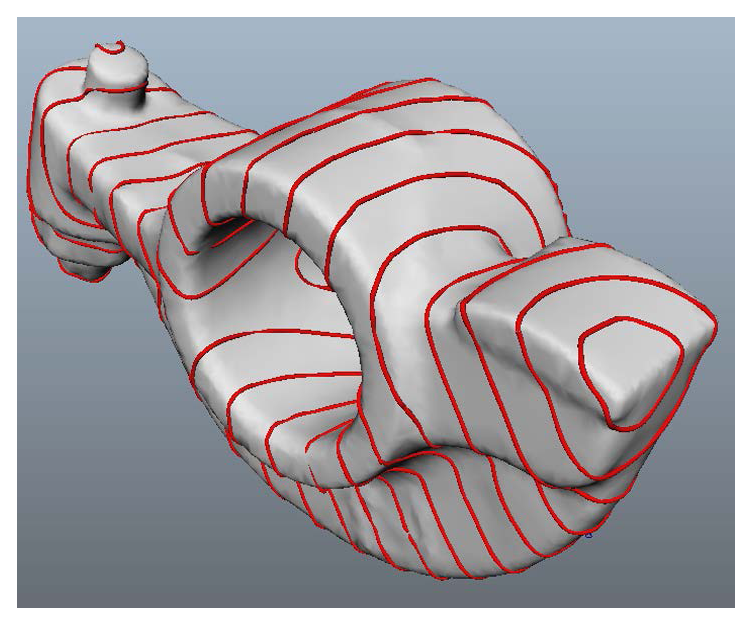
\includegraphics[width=\textwidth]{../images/geodesic_image/rocker_arm_isoline}
                \caption{isoline on rockarm}
                \label{fig:rockarm_iso}
        \end{subfigure}%        
		 
	
        \caption{Models used in geodesic computation experiments}
        \label{fig:geodesic_result}       
\end{figure}

\renewcommand{\arraystretch}{1.4}% Tighter
\renewcommand{\baselinestretch}{1.0}

\setlength{\tabcolsep}{6pt}

\begin{table}[H]
    \centering
    \small
    \begin{tabular}{|p{3.5cm}|p{2cm}|p{2.5cm}|p{2.5cm}|}
    %\begin{tabular}{|m{2.4cm}|m{1.1cm}|m{1.6cm}|m{1.6cm}|}
    %\begin{tabular}{|c|c|c|c|c|}
        \hline
        Times(sec) & Algorithm.\ref{algorithm:app_geo} & MMP app & Improved CH\_2\\
        \hline
        Hand \#V:80089\newline\#F:160000 & 6.627 & 18.762 & 13.39 \\
        \hline
        Bunny \#V:119602\newline\#F:251704 & 14.922	&  19.018 &	20.161 \\
        \hline
        Camel \#V:207266\newline\#F:414528 & 17.851 & 63.915 & 35.196 \\
        \hline
        Rockerarm \#V:241056\newline\#F:482112 & 19.944 & 85.119 & 43.114 \\
        \hline
        Jar \#V:408378\newline\#F:960516 & 56.861 & 195.09 & 93.068 \\
        \hline
        Neptune \#V:2003932\newline\#F:4007872 & 315.358 & 970.927\newline(167.992)* & 832.254\newline(689.307)* \\
        \hline
        Elephant \#V:2396060\newline\#F:4792128 & 357.435 & 1526.86\newline(194.28)* & 1962.01\newline(1524.81)* \\
        \hline
        Dragon \#V:3609455\newline\#F:7218906 & 621.892 & 2013.92\newline(229.76)* & 1281.363\newline(1008.221)* \\
        \hline
        Gargoyle \#V:5391140\newline\#F:10782288 & 1482.25 & 4649.39\newline(870.82)* & 4386.76\newline(3182.91)*\\
        \hline
        Neptune \#V:12023612\newline\#F:24047232 & 2449.44 & Out of memory 24Gb & 26822.91\newline(20175.29)* \\
        \hline
        Lucy \#V:14027872\newline\#F:28055742 & 3545.714 & Non-manifold triangles & Non-manifold triangles \\
        \hline
    \end{tabular}
    \caption[The comparison of running of presented algorithms]{The comparison of running time of Algorithm.\ref{algorithm:app_geo}, MMP app, and ICH\_2. *For several large models, the ``backtracing'' time is also showed for MMP approximation and improved ICH\_2 algorithms in brackets respectively}
    \label{table:tab_3}
\end{table}
\setlength{\tabcolsep}{6pt}
\renewcommand{\arraystretch}{1}% Tighter
\renewcommand{\baselinestretch}{1.5}

The experimental results are given in Table.\ref{table:tab_3}. Figure.\ref{fig:geodesic_result} demonstrates the shortest paths or isolines on these models that are used in Table.\ref{table:tab_3}. It can be noted that the MMP approximation and ICH\_2 algorithms can cost less time for small scale models. However, for large models, The approximate algorithm presented in this thesis is noticeably faster than others. Particularly, for large models such as Asian dragon in Figure.\ref{fig:asian_dragon}, Lucy in Figure.\ref{fig:lucy} and Gargoyle in Figure.\ref{fig:gargo} the approximate algorithm presented in this thesis is many times faster than the MMP approximation and ICH\_2. 

Moreover, It can be observed that the ``backtracing'' takes up too much time in MMP and ICH algorithms, in particular, the ``backtracing'' occupies most of the running times for the large models in ICH\_2. This further verifies The approximate algorithm presented in this thesis is appropriate for tracing accurate geodesic paths on large models.